\documentclass{article}

\title{Laborjournal zur Herstellung von Gummibärchen und Seife}
\author{Oliver Schütz}
\date{\today}

\usepackage[utf8]{inputenc}
\usepackage{hyperref}
\usepackage{graphicx}
\usepackage{amsmath}
\usepackage{array}


\begin{document}
    \maketitle

    \section{Gummibärchen aus Pektin}

    \subsection{Ziel}
    Ziel ist die Herstellung von Gummibärchen (essbar wenn Möglich) unter Verwendung von Pektin als Geliermittel.

    \subsection{Theorie}
    Pektin ist ein Geliermittel, das aus Äpfeln gewonnen wird.
    Es kann zusammen mit Zucker Lösungen verdicken oder sogar fest werden lassen.
    In Kombination mit Zucker und Säure bilden sich bei Erwärmung Pektin-Gele, die die Grundlage für Gummibären bilden.


    \subsection{Durchführung}

    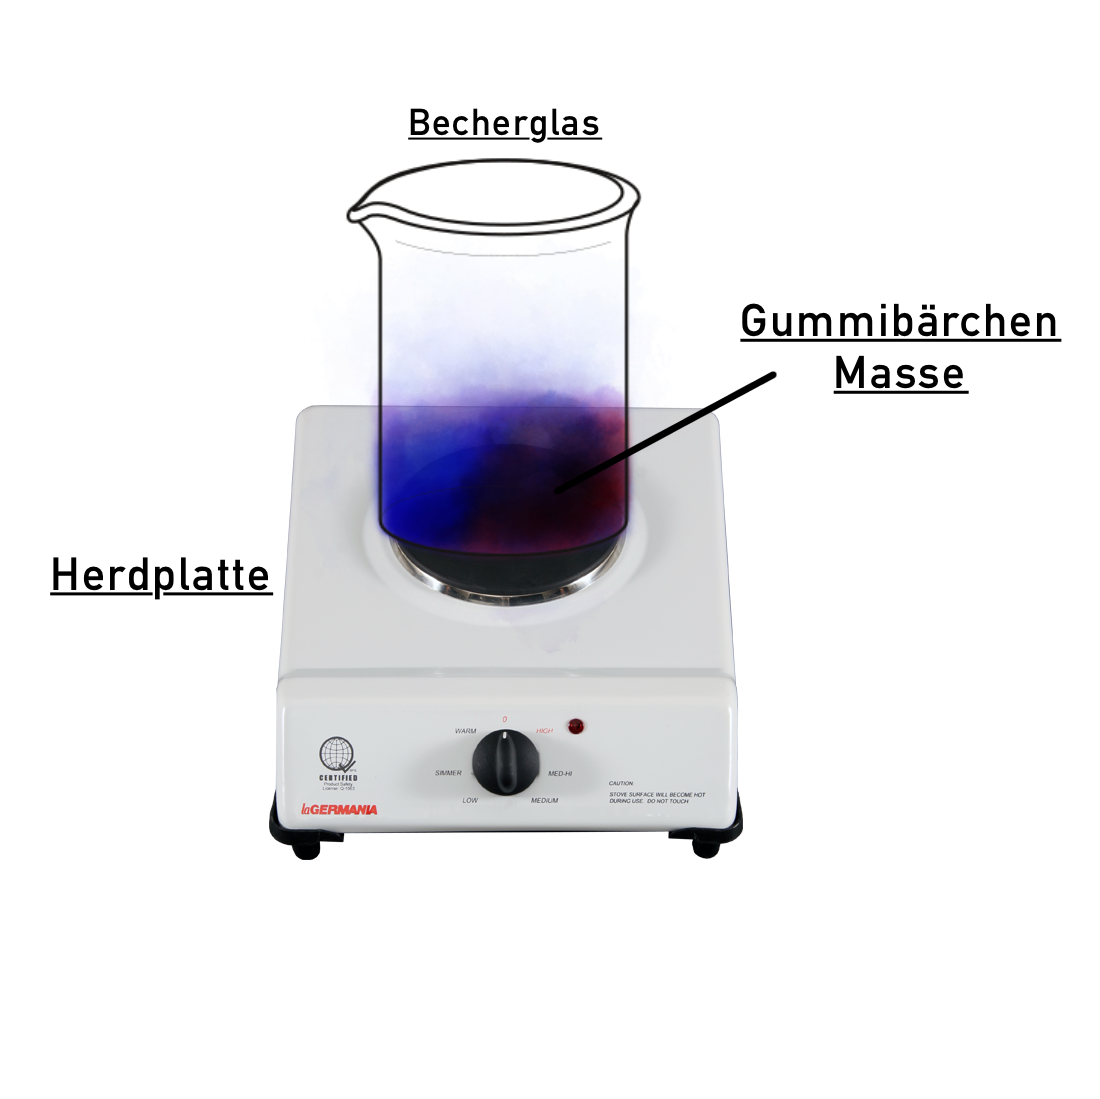
\includegraphics[width=0.8\textwidth]{Gummi.png} \\

    \begin{itemize}
        \item Herstellung von Invertzucker: 100 g Saccharose, Prise Weinsäure, 50 g Wasser mischen und 30 Minuten bei 70 °C erhitzen.
        \item Zitronensäurelösung: 5g Zitronensaure in 5g Wasser lösen.
        \item Mischung aus 0,6 g Natriumcitrat, 7,5 g Apfelpektin und 30 g Saccharose in 60-ml (50°C) Wasser geben und umrühren.
        \item 25 g Saccharose und Invertzucker in Pektinmischung einrühren und auf 100°C erhitzen.
    \end{itemize}
    Nun noch Aromen und dann Farbstoffe mit Zitronensäurelösung hinzugeben.
    Die Formen mit Stärke bestäuben und die Masse einfüllen.

    \subsection{Beobachtungen}
    Zu Beginn war die Masse recht flüssig, da das Pektin mit Apfelsäure vertauscht wurde.
    Als im Nachgang noch Pektin hinzugefügt wurde, wurde die Masse fester.
    Es haben sich während des Erhitzens Blasen gebildet, die auch bis Ende nicht verschwunden sind.
    Die Masse konnte leicht in die Formen gefüllt werden, ist jedoch schnell zähflüssig geworden.

    \subsection{Fazit}
    Auch wenn ein Vielfaches an Apfelsäure verwendet wurde, waren die Gummibären noch gut essbar,
    etwa so sauer wie Center-Shocks.
    Die Konsistenz der Gummibären war sehr weich und leicht brüchig.

    \subsection{Erklärung}
    Die Blasen entstehen durch die Verdampfung des Wassers.
    Die Masse wird zähflüssig, da das Pektin mit dem Zucker reagiert und ein Gel bildet.

    \subsection{Verbesserungsvorschläge}
    Ursachen für Konsistenz und Geschmack:

    \begin{itemize}
        \item Zu wenig Pektin
        \item Zu hoher Wasseranteil
        \item Zu kurze Kochzeit
    \end{itemize}
    Für festere Gummibären ist mehr Pektin, weniger Wasser und längere Kochzeit bei höherer Temperatur eine Option.
    Auch langsames Abkühlen und längeres Trocknen würde die Konsistenz verbessern.
    Es sollte zudem genau darauf geachtet werden, die richtige Zutat zu verwenden.

    \newpage
    \section{Seifenherstellung}

    \subsection{Ziel}
    Herstellung von Seife aus Kokosfett, Rapsöl und Natriumhydroxid.

    \subsection{Theorie}
    Seifen entstehen durch die alkalische Verseifung von Fetten unter Abspaltung von Glycerin.

    \subsection{Durchführung}
    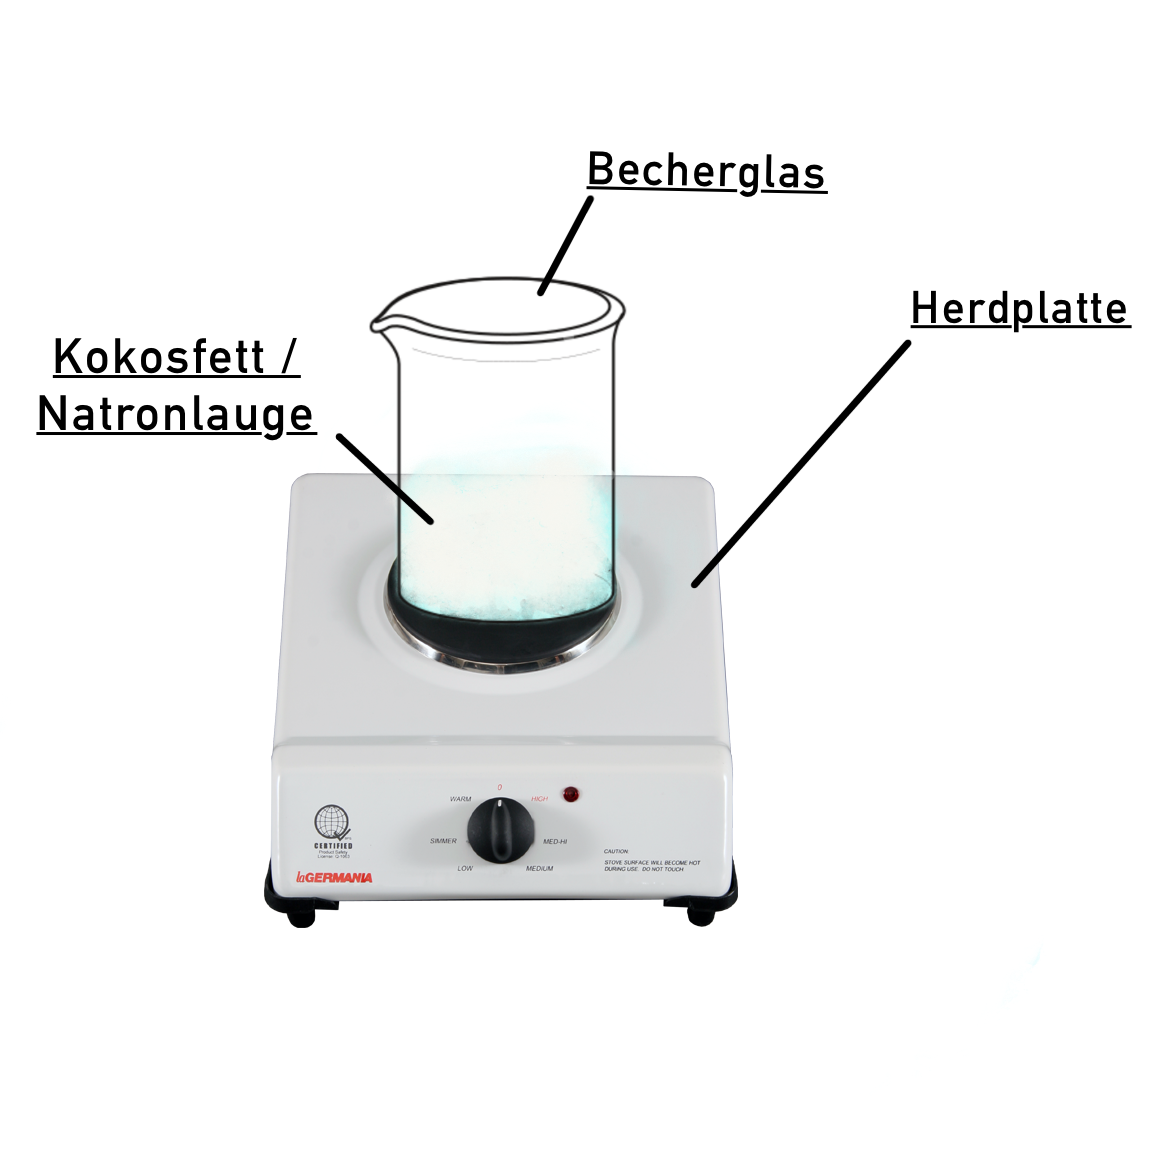
\includegraphics[width=0.8\textwidth]{Seife.png} \\
    Zuerst wird 100g Kokosfett mit 100g Olivenöl in einem Becherglas püriert.
    In einem seperaten Becherglas, wird Natriumhydroxid in Wasser gelöst.
    Anschließend wird beides in einem neuen Becherglas bei heißer Herdplatte gerührt.

    \subsection{Berechnung}


    \begin{align*}
        \text Rapsöl = 100g \\
        \text Kokosfett = 100g \\
        \text{Verseifungszahl}_{\text{Rapsöl}} & = 0,1354 \\
        \text{Verseifungszahl}_{\text{Kokosfett}} & = 0,1830 \\
        m_{\text{NaOH}} & = 13,54\text{g} + 18,30\text{g} \\
        m_{\text{NaOH}} & = 31,84\text{g}  \\
        m_{\text{Wasser}} & = \frac{1}{3} \cdot 200\text{g} = 67\text{g}
    \end{align*}

    \subsection{Beobachtungen}
    Beim Lösen des Natriumhydroxids wurde das Becherglas spürbar warm und es hat sich ein Gas gebildet.
    Als alles verrührt wurde, wurde die Masse über Zeit zäh und fing an zu kleineren Klumpen zu werden.


    \subsection{Erklärung}
    Es sind Klumpen entstanden, weil zu lange gerührt wurde.
    Es könnte auch an einer falsch eingestellten Temperatur gelegen haben.

    \subsection{Reflexion}
    Um ein besseres Ergebnis zu erhalten, könnte weniger gerührt werden und das Mischverhältnis noch überdacht werden.
\end{document}

